\section{Background}
\label{sec:background}

Container technology has gain tremendous popularity~\cite{iron-io-300-million}
since it enables a fast and easy way to package, distribute and deploy
applications and services.  

Containers are essentially processes, but they use mechanisms as {\tt
chroot}~\cite{chroot} to provide namespace isolation.  The dependencies of
containerized applications are bundled together with the application, making
them highly portable: they can be easily distributed and deployed~\cite{docker}.
Compared to VMs, containers are much more lightweight and can be initialized
much faster~\cite{xxx}.  manner. Containers can be deployed both within a VM or
on bare metal. Containers are supported by both Linux an Windows operating
system.  Docker~\cite{docker} is perhaps the most popular container management
system, although there are many others as well~\cite{coreos,kubernetes}.

Most containerized applications are usually composed from multiple containers.
For example, each mapper and reducer node in Hadoop \cite{hadoop} is an
individual container. A modern web service with multiple layers (load balancers,
web servers, in-memory caches and backend databases) is deployed with multiple
containers in each layer.  These containers are usually deployed into a
multi-host server cluster, and the deployment is usually controlled by a cluster
orchestrator, e.g. Mesos~\cite{mesos} or Kubernetes~\cite{xxx}.  Such architecture makes it easier to
upgrade the nodes or mitigate failures, since a stopped container can be quickly
replaced by a new one on the same or a different host.  Working as a single
application, containers need to exchange data, and the network performance has a
significant impact on the overall application performance~\cite{coflow-etc.}

Depending on whether containers run on bare-metal hosts or VM hosts, there are
four cases any container networking solution must handle. These cases are
illustrated in Figure~\ref{fig:deploy-cases}.  For maximum portability,
containers today often use overlay networks as shown in Figure~\ref{fig:overlay}.
A number of software solutions are available to provide this overlay fabric,
such as Weave~\cite{weave} and Calico~\cite{calico}. In these solutions, the
host (i.e.  the server or the VM) runs software router. The router connect to
the NIC of the host. It also connects with the virtual interfaces of the
containers on the host via a software bridge. It performs appropriate tunneling
(encapsulation and decapsulation) to move traffic between the physical network
and the overlay fabric. The router uses standard networking protocols like BGP
to connect with software routers on other hosts. Containers send and receive IP
packets via this overlay, and hence are agnostic to location of other containers
they are communicating with.

The CPU overhead of processing packets in the software bridge, as well as in the
software router (for off-host communication) is the primary bottleneck to the
performance of this overlay network, as illustrated in
Figure~\ref{fig:mot_bw_cpu}. The figure shows throughput and CPU utilization of
two containers, running iPerf, deployed on two different physical servers and
connected via overlay routing using Weave~\cite{weave}. The throughput tops off
at 20Gbps, because both the sender and the receiver CPUs are fully utilized.

\begin{figure} [t]
	\centering   
	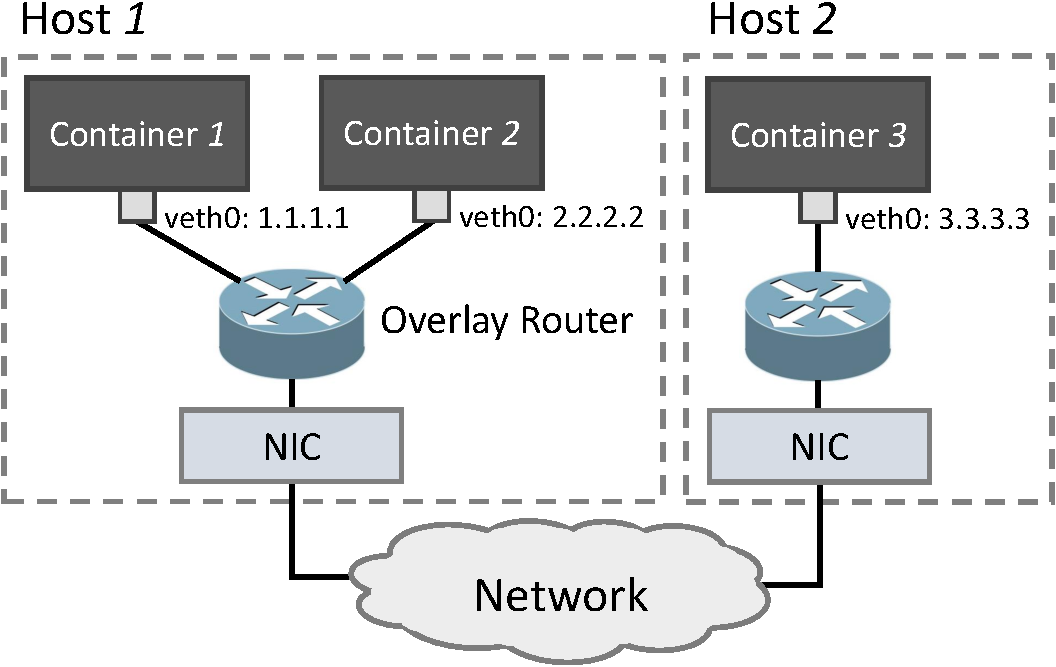
\includegraphics[width=0.8\linewidth]{figures/overlay-2.pdf}   
	\caption{\label{fig:overlay} The design of existing container overlay networks (Weave).}   
\end{figure}   

\begin{figure}[t]
\centering 
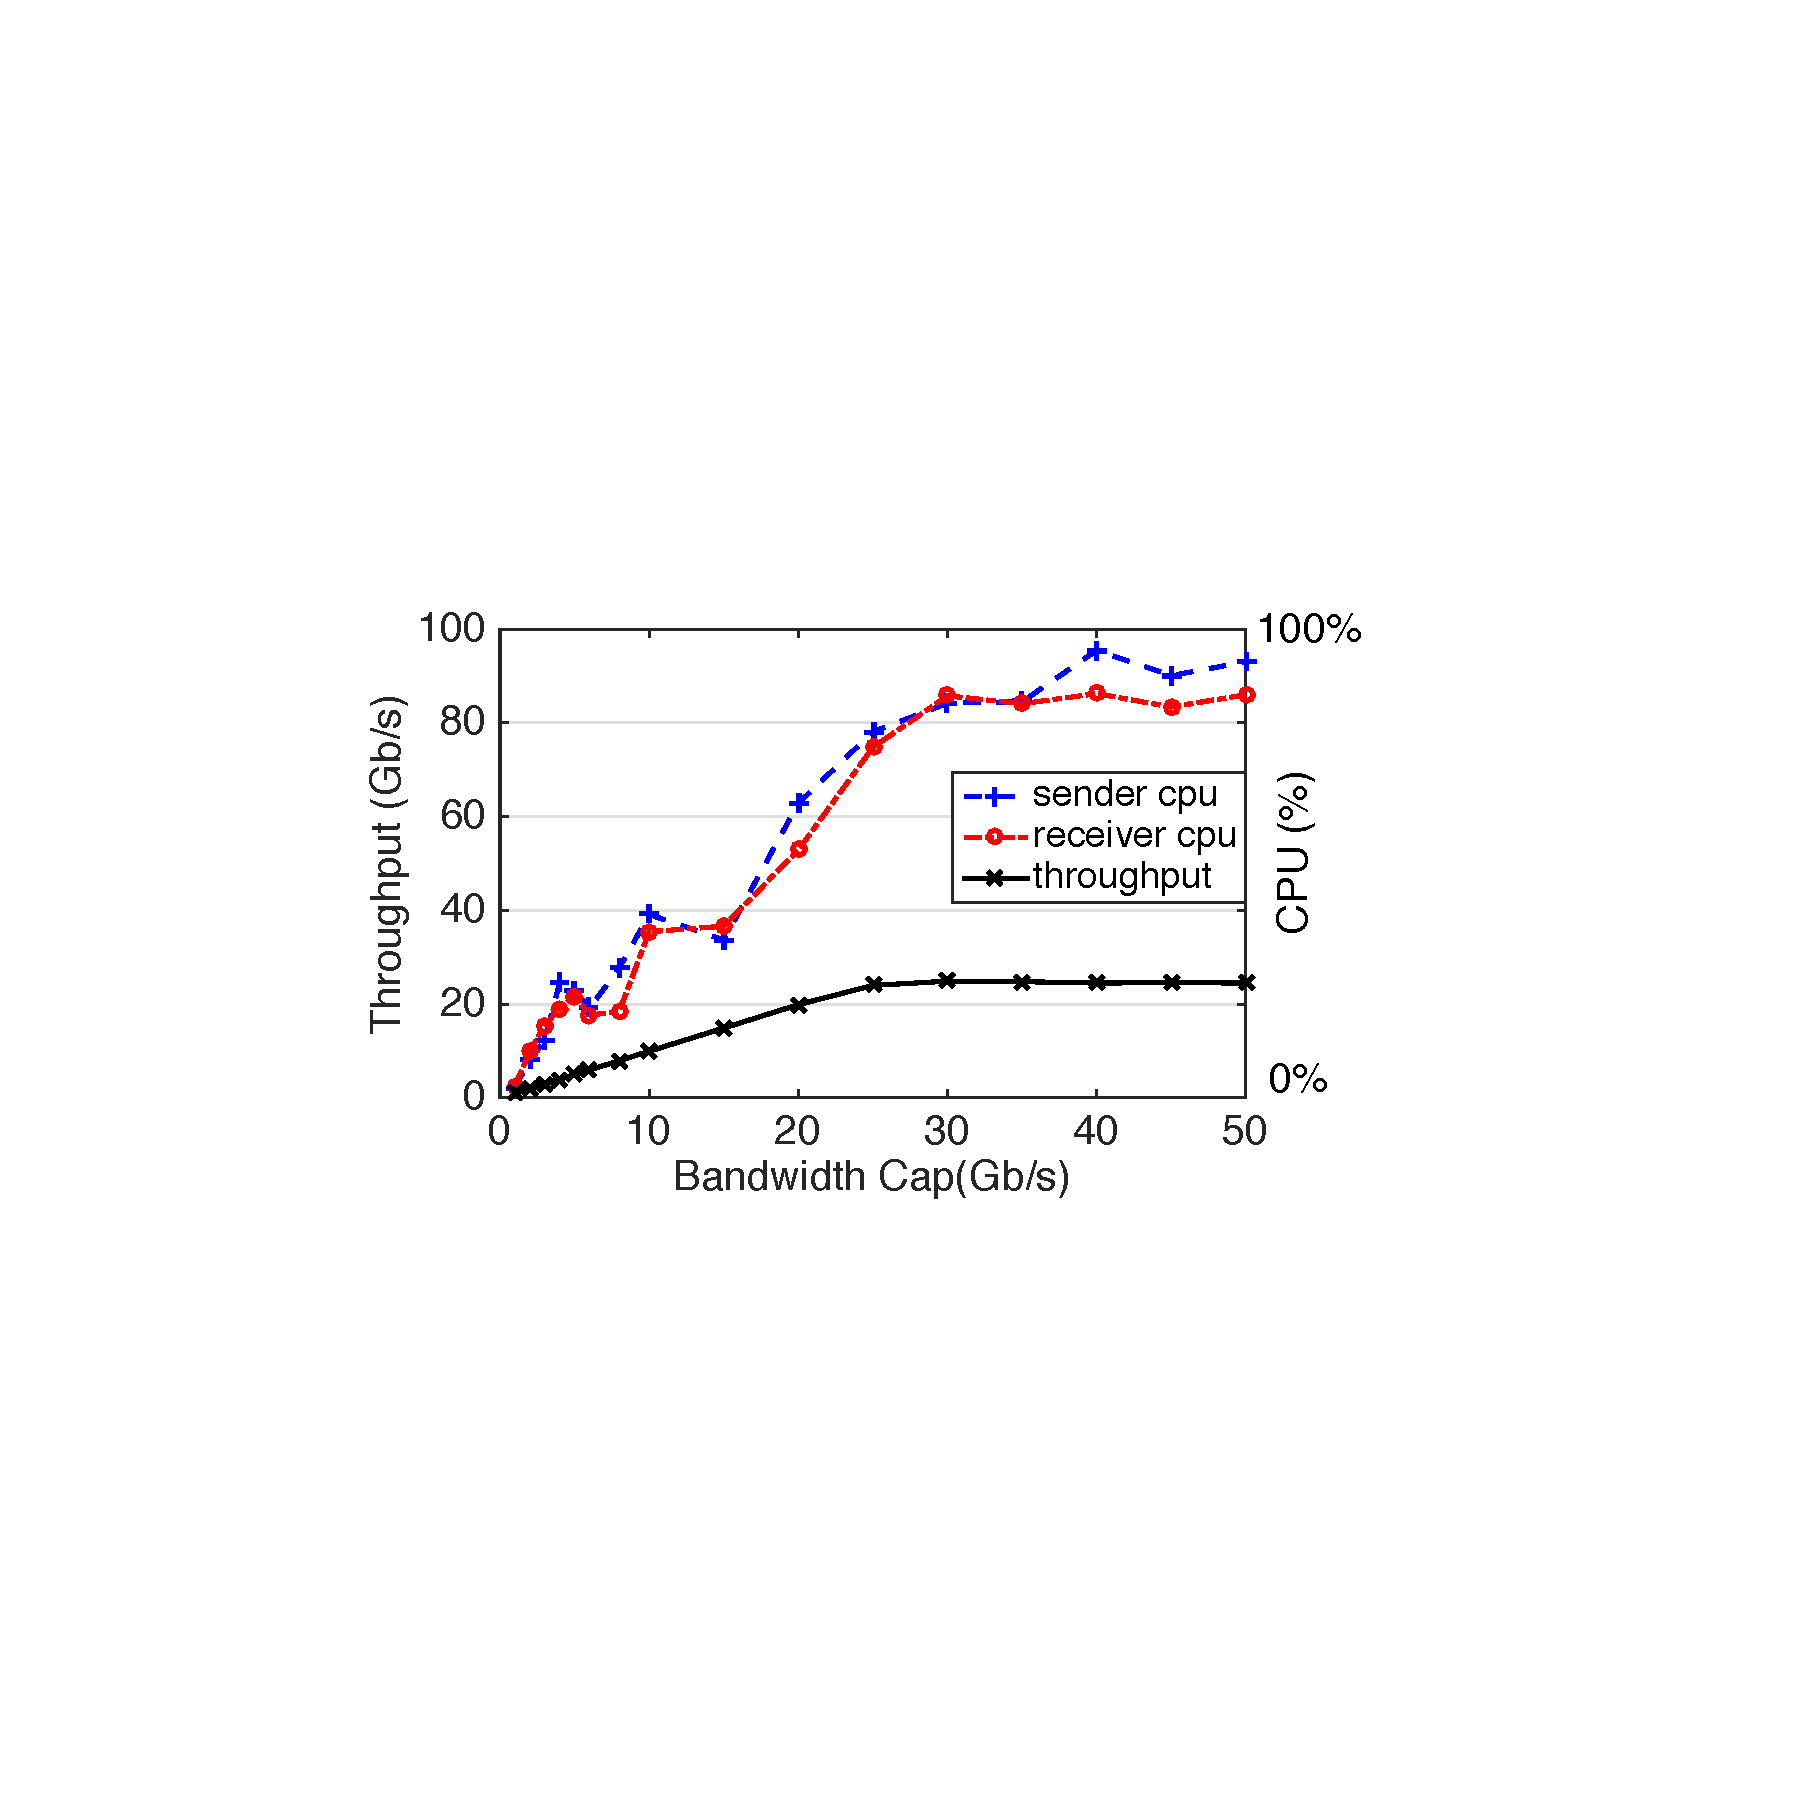
\includegraphics[width=0.5\textwidth]{figures/motivation/mot_bw_cpu.pdf}      
\label{fig:mot_bw_cpu}
\caption{CPU limits overlay networking throughput}
\end{figure}
